
\begin{center}
\Huge
Mere om cirkler
\end{center}
\section*{Kvadratkomplettering}
\stepcounter{section}

Får vi ligningen for en cirkel med radius $r$ og centrum i $(x_0,y_0)$, så kan det være, at den ikke er på formen 
\begin{align}\label{eq:1}
(x-x_0)^2 + (y-y_0)^2 = r^2,
\end{align}
men at parenteserne i stedet er hævet, så ligningen er på formen
\begin{align}\label{eq:2}
x^2+x_0^2-2xx_0 + y^2+y_0^2-2yy_0 = r^2
\end{align}
Idéen er nu at vi skal kunne \textit{kvadratkomplettere}, så vi kan omskrive ligningen fra formen $\eqref{eq:2}$ til formen $\eqref{eq:1}$. Lad os betragte et eksempel.
\begin{exa}
En cirkel har ligningen 
\[
	x^2-4x+y^2+8y+11=0,
\]
og vi vil gerne bestemme centrum og radius for denne cirkel. Vi skal derfor omskrive ligningen til formen \eqref{eq:2} og derefter til \eqref{eq:1}. I ligningen har vi leddene $-4x = -2xx_0$, så $x_0$ må være $2$. Tilsvarende har vi, at $8y = -2yy_0$ så $y_0 = -4$. I ligningen mangler vi leddene $x_0^2 = 4$ og $y_0^2 = 16$, så dem lægger vi til på begge sider af lighedstegnet:
\begin{align*}
x^2-4x+y^2+8y+11=0 \ \Leftrightarrow \ x^2-4x + 4 +y^2+8y+11 + 16=20,
\end{align*}
Vi flytter nu det overskydende $11$ over på højre side af lighedstegnet og får
\begin{align*}
x^2-4x+4+y^2+8y+16 = 9.
\end{align*}
Nu er ligningen på formen \eqref{eq:2}, og vi omskriver derfor til formen \eqref{eq:1}:
\begin{align*}
(x-2)^2+(y+4)^2= 3^2,
\end{align*}
og centrum ligger derfor i $(2,-4)$ og radius af cirklen er $r=3$. 
\end{exa}

\section*{Tangenter til cirkler}
\stepcounter{section}
Hvis vi kender et punkt $P(x_0,y_0)$ på en cirkel, så kan vi bestemme en tangent til cirklen i dette punkt, hvis vi kender centrum for cirklen. Vi kunne i princippet sagtens bestemme en formel for ligningen for tangenten, men lad os for intuitionens skyld bestemme ligningen gennem et eksempel.
\begin{exa}
En cirkel har centrum i $C(2,1)$ og et punkt $P(3.41,2.41)$ ligger på cirklen. Vi ønsker at bestemme ligningen for tangenten $l$ til cirklen i dette punkt. Vi udnytter, at vektoren 
\begin{align*}
\vv{PC} = 
\begin{pmatrix}
2-3.41 \\ 1-2.41
\end{pmatrix} =
\begin{pmatrix}
-1.41 \\ -1.41
\end{pmatrix}
\end{align*}
er en normalvektor til $l$. Desuden kender vi et punkt $l$ skærer igennem - $P$. Derfor kan vi anvende formlen for linjens ligning, der kræver en normalvektor 
\begin{align*}
\vv{n} = \begin{pmatrix}
a \\ b
\end{pmatrix}
\end{align*} 
og et punkt på linjen $P(x_0,y_0)$. Dette giver ligningen
\begin{align*}
a(x-x_0) + b(y-y_0) = 0 \ \Leftrightarrow \ -1.41(x-3.41) -1.41(y-2.41) = 0
\end{align*}
for tangenten for cirklen i punktet $P$. 
\end{exa}

\section*{Skæringer mellem linje og cirkel}
\stepcounter{section}
Skal vi finde skæringen mellem en linje og en cirkel, så er fremgangsmåden ikke overraskende meget lig metoden til at finde skæringer mellem linjer. Vi ser på et eksempel.
\begin{exa}
Lad os igen betragte cirklen med ligningen 
\begin{align*}
x^2-4x+y^2+8y+11 = 0.
\end{align*}
Vi skal bestemme de to punkter, hvor linjen $l$ med ligningen 
\begin{align*}
y = -x-2
\end{align*}
skærer cirklen. Derfor indsætter vi udtrykket for $y$ fra linjens ligning på $y$'s plads i cirklens ligning og får:
\begin{align*}
x^2-4x+y^2+8y+11 = 0 \  &\Leftrightarrow \  x^2-4x+(-x-2)^2+8(-x-2)+11=0\\
&\Leftrightarrow \ 2x^2-8x-1 = 0.
\end{align*}
Vi løser denne andengradsligning med diskriminantformlen for får
\begin{align*}
x &= \frac{8\pm\sqrt{64-8}}{4}\\
&= 2\pm \frac{3\sqrt{2}}{2}.
\end{align*}
Vi indsætter nu dette i formlen for $y$ for at få $y$-værdierne for skæringerne og får
\begin{align*}
y = -(2\pm \frac{3\sqrt{2}}{2}) - 2 = -4 \mp \frac{3\sqrt{2}}{2}.
\end{align*}
De to skæringspunkter er derfor
\begin{align*}
(2+ \frac{3\sqrt{2}}{2},-4 - \frac{3\sqrt{2}}{2}) \approx (4.1213,-6.1213)
\end{align*}
og
\begin{align*}
(2- \frac{3\sqrt{2}}{2},-4 + \frac{3\sqrt{2}}{2}) \approx (-0.1213,-1.8787)
\end{align*}
Vi kan se linjen $l$ og cirklen på Fig. \ref{fig:cirkel}.
\begin{figure}[H]
\centering
\resizebox{0.7\textwidth}{0.7\textwidth}
{
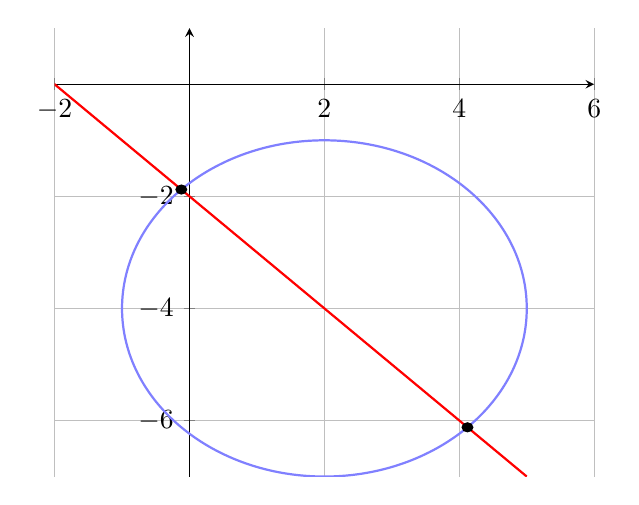
\begin{tikzpicture}
\begin{axis}[axis lines = middle, xmin = -2, xmax = 6, ymin = -7, ymax = 1,
grid = both
]
\draw[color = blue!50, thick]  (axis cs:2,-4) circle (3);
\addplot[color = red, thick] {-x-2};
\draw[fill, black] (axis cs:4.1213,-6.1213) circle (0.08);
\draw[fill, black] (axis cs:-0.1213,-1.8787) circle (0.08);
\end{axis}
\end{tikzpicture}
}
\caption{Skæringer mellem cirkel og linje}
\label{fig:cirkel}
\end{figure}
Vi kan se, at skæringen mellem cirklen og linjen er fundet korrekt.
\end{exa}

\section*{Opgave 1}
Følgende er ligninger for cirkler. Brug kvadratkomplettering til at bestemme centrum og radius for cirklerne. Undersøg i Geogebra, om det er den korrekte cirkel, du har bestemt.
\begin{align*}
&1) \ x^2-2x+y^2-2y+1=0   &&2) \  x^2+4x+y^2-6y+9=0   \\
&3) \ x^2+6x+y^2+12y+29=0  &&4) \ x^2-8x+y^2+10y+5=0   \\
\end{align*}
\section*{Opgave 2}
\begin{enumerate}[label=\roman*)]
\item En cirkel har centrum i $(0,0)$. Punktet $P(0.42,0.91)$ ligger på cirklen. Bestem ligningen for tangenten til cirklen i punktet $P$. Undersøg i Geogebra, om du har fundet den korrekte ligning.
\item En cirkel har centrum i $(2,-3)$. Punktet $P(1.37,-4.9)$ ligger på cirklen. Bestem ligningen for tangenten til cirklen i punktet $P$. Undersøg i Geogebra, om du har fundet den korrekte ligning.
\item En cirkel har centrum i $(-4,4)$. Punktet $(0,0)$ ligger på cirklen. Bestem ligningen for tangenten til cirklen i punktet $P$. Undersøg i Geogebra, om du har fundet den korrekte ligning.
\end{enumerate}

\section*{Opgave 3}
\begin{enumerate}[label=\roman*)]
\item En cirkel har centrum i $(1,1)$ og radius $2$ Bestem skæringen mellem denne cirlen og linjen med ligningen $y=x$.
\item En cirkel har centrum i $(0,0)$ og radius $5$ Bestem skæringen mellem denne cirlen og linjen med ligningen $y=2x-1$.
\end{enumerate}

\section*{Opgave 4}
En linje har normalvektor $(1,2)$ og skærer gennem punktet $(1,1)$. En cirkel har centrum i $(1,1)$ og radius $4$. Bestem skæringen mellem linjen og cirklen og bestem derefter ligningen for tangenterne til cirklen i skæringspunkterne. 



